\section{Seismische Wellen und Seismik}

Ausgelöst durch zum Beispiel Stöße auf die Erdoberfläche oder Erdbeben, kommt es auf der Erde zur Bewegung der Partikel in der Erdoberfläche. Diese Bewegung breitet sich vom Ursprungsort in alle Richtungen aus. Es wird von seismischen Wellen gesprochen. Abhängig von der Partikelbewegung im Untergrund, gibt es longitudinale und transversale Wellen.

Bei longitudinal polarisierten Wellen schwingen die Partikel parallel zur Ausbreitungsgeschwindigkeit der Welle. Sie werden auch P-Wellen oder Kompressionswellen genannt und haben in homogenen isotropen Medien eine Geschwindigkeit von
\begin{equation}
 \q{v}{P}=\sqrt{\frac{\kappa+\frac{4}{3}\mu}{\rho}} \comma
\end{equation}
wobei $\kappa$ das Volumenkompressionsmodul und $\rho$ die Massendichte ist.

Bei senkrechter Partikelbewegung zur Ausbreitungsgeschwindigkeit ist die Welle transversal polarisiert. Sie Wird auch A-Welle oder Scherwelle genannt und hat in homogenen isotropen Medien eine Ausbreitungsgeschwindigkeit von
\begin{equation}
 \q{v}{S}=\sqrt{\frac{\mu}{\rho}} \fullstop
\end{equation}
Da in Flüssigkeiten $\mu=\e{0}{Pa}$ gilt, können sich in diesen keine Scherwellen ausbreiten.

In der Seismik werden diese Wellen durch zum Beispiel einen Hammer (Hammerschlagseismik) künstlich ausgelöst. In verschiedenen Abständen zur Quelle wird mit  Geophonen die Bodenbewegung gemessen und daraus kann dann auf die Ausbreitungsgeschwindigkeit der Wellen im Untergrund geschlossen werden. Es werden bei der Refraktionsseismik nur die Ersteinsätze betrachtet, es wird also nur die P-Wellengeschwindigkeit $\q{v}{P}$ analysiert, weil diese Größer ist als die S-Wellengeschwindigkeit. Die Ersteinsätze erfolgen also immer durch P-Wellen.

\section{Snelliussches Brechungsgesetz und refraktierte Welle} %oder Strahlenseismik???

Wenn die Wellenlänge der Welle sehr viel kleiner als der Abstand zwischen Quelle und Empfänger ist, können die Wellen als Strahl beschrieben werden. Trifft eine Welle auf eine Schichtgrenze (Grenze zwischen Materialien mit unterschiedlichen Ausbreitungsgeschwindigkeiten), wird sie sowohl reflektiert, als auch in das andere Medium gebrochen. Für die reflektierte Welle gilt das Snelliussche Brechungsgesetz
\begin{equation}
 \frac{\sin(\alpha_1)}{\sin(\alpha_2)}=\frac{v_1}{v_2}\fullstop
\end{equation}
$\alpha_1$ ist dabei der der Einfallswinkel zum Lot hin gemessen und $v_1$ die Geschwindigkeit im Medium, in dem der Strahl auf die Grenzfläche einfällt. $\alpha_2$ ist der Ausfallswinkel zum Lot hin gemessen und $v_2$ die Geschwindigkeit im Medium, in das der Strahl hinein gebrochen wird.

Falls $v_2>v_1$ gilt, ist auch $\alpha_2>\alpha_1$. Sobald $\alpha_2=90^\circ$ gilt, kommt es statt zur Reflektion zur Refraktion. Dies passiert ab dem kritischen Winkel
\begin{equation}
 \sin(\q{\alpha}{k}) =\frac{v_1}{v_2} \fullstop
\end{equation}
Eine Welle, die im kritischen Winkel auf die Grenzfläche auftritt, läuft mit der Geschwindigkeit $v_2$ an der Grenzfläche entlang und strahlt permanent ebenfalls unter dem kritischen Winkel Wellen nach oben ab, die dann wieder die Geschwindigkeit $v_1$ des oberen Mediums haben.

\section{Laufzeitdiagramme}

% Basalt: $\q{v}{P}>\eb{4000}{m}{s}$
Im Seismogramm werden die Einsätze der Wellen abgelesen. Dann können die Laufzeiten $t$ gegen die Geophondistanz $x$ vom Schussort aufgetragen werden. Die erhaltene Kurve heißt Laufzeitdiagramm. Die weitere Auswertung erfolgt aus diesen Diagrammen, wobei nur die Ersteinsätze ausgewertet werden. Zuerst wird der Ersteinsatz durch die direkte Welle (Kompressionswelle, die an Erdoberfläche entlang läuft) gebildet und ab einer bestimmten Geophondistanz überholt die refraktierte Welle die direkte Welle, so dass der Ersteinsatz nun durch diese erfolgt. Dies ist auch in Abbildung ??? zu sehen.
% Auswertung (eine Schicht, zwei Schichten, geneigte Schichten, Verfahren der Verzögerungszeiten) ???

\section{Auswertung bei zwei schichten über dem Halbraum}
???Muss noch geschrieben werden???

Der Strahlengang und das Laufzeitdiagramm für diesen Fall sind in Abbildung \ref{zweiSchichten} zu sehen.

\begin{figure}
 \centering
 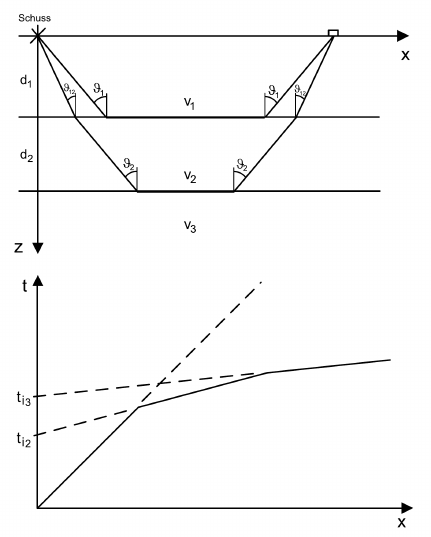
\includegraphics[width=0.5\textwidth]{fig/zweischichten}
 \caption[Strahlengang und Laufzeitdiagramm für den Fall von zwei homogenen Schichten über einem homogenen Halbraum]{Strahlengang und Laufzeitdiagramm für den Fall von zwei homogenen Schichten über einem homogenen Halbraum \cite{skript}}
 \label{fig:zweiSchichten}
\end{figure}

Bei der Beschreibung der Formel wird die Notation des Skripts \cite{skript} verwendet. Hin- und Rückschuss haben von ihrem Nullpunkt aus gesehen den gleichen Verlauf. Aus der ersten Geraden folgt die Laufzeit der direkten Welle
\begin{equation}
 t_1=\frac{x}{v_1} \fullstop
\end{equation}
Aus der zweiten Gerade folgt die Laufzeit
\begin{equation}
 t_2=\frac{x}{v_2}+\frac{2d_1\cos(\vartheta_1)}{v_1}=\frac{x}{v_2}+t_{i2}
\end{equation}
der ersten refraktierten Welle. Die Intercept-Zeit
\begin{equation}
\label{eq:ti2}
 t_{i2}=\frac{2d_1\cos(\vartheta_1)}{v_1}
\end{equation}
ist die theoretische Ersteinsatz-Zeit der refraktierten Welle. Der dritte Abschnitt ist dann die Laufzeitgerade der am Halbraum refraktierten Welle
\begin{equation}
 t_3=\frac{x}{v_3}+\frac{2d_1}{v_1}\cos(\vartheta_{12})+\frac{2d_2}{v_2}\cos(\vartheta_2)=\frac{x}{v_3}+t_{i3} \fullstop
\end{equation}
Mit der Intercept-Zeit
\begin{equation}
\label{eq:ti3}
 t_{i3}=\frac{2d_1}{v_1}\cos(\vartheta_{12})+\frac{2d_2}{v_2}\cos(\vartheta_2)\comma
\end{equation}
dem kritischen Winkel 
\begin{equation}
 \sin(\vartheta_2)=\frac{v_2}{v_3}
\end{equation}
für die zweite Schichtgrenze und dem Ausfallswinkel
\begin{equation}
 \sin(\vartheta_{12})=\frac{v_1}{v_2}\sin(\vartheta_2)=\frac{v_1}{v_3}
\end{equation}
an der ersten Schichtgrenze eines von unten nach oben laufenden Strahls, der die zweite Schichtgrenze unter dem Winkel $\vartheta_2$ verlassen hat.

Die Ersteinsatz-Laufzeitkurven können dann folgendermaßen ausgewertet werden: Die Geschwindigkeiten $v_1$, $v_2$ und $v_3$ werden aus den Steigungen der drei geraden Abschnitte der Laufzeitkurven bestimmt. Sie entsprechen dem Kehrwert der Steigungen. Die Intercept-Zeiten sind die $t$-Achsenabschnitte der zweiten bzw. dritten Geraden. Sie können aus dem Laufzeitdiagramm abgelesen werden. Die relevanten Winkel
\begin{align}
 \vartheta_1=\arcsin\left(\frac{v_1}{v_2}\right) \\
 \vartheta_2=\arcsin\left(\frac{v_2}{v_3}\right) \\
 \vartheta_{12}=\arcsin\left(\frac{v_1}{v_3}\right)
\end{align}
werden aus den Geschwindigkeiten berechnet. Die Schichtmächtigkeiten $d_i$ werden dann letztlich durch Umstellen der Gleichungen \eqref{eq:ti2} und \eqref{eq:ti3} zu
\begin{align}
 d_1&=\frac{t_{i2}v_1}{2\cos(\vartheta_1)} \\
 d_2&=\frac{v_2}{2\cos(\vartheta_2)}\left(t_{i3}-\frac{2d_1}{v_1}\cos(\vartheta_{12})\right)
\end{align}
berechnet.

\section{Messinsrumente}

Der Messaufbau dieser Seismik-Versuche ist in Abbildung ??? dargestellt. Als Signalquelle dient ein Vorschlaghammer (Hammerschlagseismik) oder eine Verpuffung (schwache Explosion), die die seismischen Wellen anregt. Die Bodenbewegung wird mit Geophonen gemessen. Diese bestehen aus einem Magneten, der Fest mit deren Gehäuse verbunden ist und um den eine Spule frei schwingen kann. Eine Bodenbewegung versetzt die Spule und den Magneten in Relativbewegung zueinander, wodurch eine elektrische Spannung in der Spule induziert wird. Diese Spannung ist proportional zur Bodenschwinggeschwindigkeit und wird vom Digitalisierer (in diesem Versuch wird eine Geode genutzt) abgetastet, gepuffert und dann an das Laptop weitergeleitet, welches die Messwerte ausgibt und aufzeichnet. Die Signale werden im seismische Dateiformat SEG-Y-Format auf der Festplatte abgespeichert.

Der Trigger gibt der Software auf dem Laptop das Startsignal zur Aufzeichnung der Messung. Dies geschieht genau dann, wenn die Quelle ausgelöst wird. Er ist an der Quelle angebracht und an einer Diode angeschlossen, die das Triggersignal an andere Geoden und die Software weiterleitet.  

Wird die Hammerschlagseismik verwendet, werden pro Schusspunkt oft mehrere Schläge durchgeführt und die Seismogramme danach aufsummiert. Die Signale werden dadurch deutlicher, weil sich die Nutzsignale konstruktiv addieren, was jedoch für die Störsignale (Rauschen) nicht der Fall ist. Dieses Prinzip wird Stapelung genannt. Bei längeren Messprofilen wird die Verpuffungsquelle S.I.S.Sy verwendet, weil sie eine höherer Energie als der Hammerschlag aufweist und so ein Schuss ausreicht.

% \begin{figure}
%  \centering
%  \includegraphics[width=\textwidth]{fig/}
%  \caption{}
%  \label{fig:}
% \end{figure}